\subsection{\textgreek {Επεξεργασία συλλογής}}
\textgreek{
    Η αρχική μορφή των δεδομένων ήταν τύπου $json$.
    Τα δεδομένα μετατράπηκαν
    σε μορφή τύπου $csv$, με σκοπό την ταχύτερη εισαγωγή τους στη βάση δεδομένων.

    Για τη μετατροπή χρησιμοποιήθηκε το πρόγραμμα $jq$.
    Το $script$ για την
    \\ μετατροπή είναι το $src/main/resources/json\_to\_csv.sh$
}
\lstset{
basicstyle=\footnotesize,
showstringspaces=false,
commentstyle=\color{red},
keywordstyle=\color{blue},
breakatwhitespace=false,
breaklines=true
}
\begin{lstlisting}[language=bash]
    #!/bin/bash

    # example usage of `jq` for exporting to tsv
    jq -r '[.business_id, .name, .latitude, .longitude, .city, .stars, .review_count, .address, .postal_code, .categories] | @tsv' \
    business.json                               \
    | tr "\"" "'"                               \
    > businesses.tsv

    jq -r '[.review_id, .business_id, .stars, .date, .text, .useful, .funny, .cool] | @tsv' \
    review.json                               \
    | tr "\"" "'"                               \
    > reviews.tsv

    jq -r '[.text, .date, .compliment_count, .business_id] | @tsv' \
    tip.json                               \
    | tr "\"" "'"                               \
    > tips.tsv

\end{lstlisting}


\subsection{\textgreek{Βάση Δεδομένων}}
\textgreek{
    Με στόχο την καλύτερη και ευκολότερη διαχείρηση των δεδομένων σε μια
    πιο δομημένη μορφή, δημιουργήθηκε σχεσιακή βάση δεδομένων.

    Το σύστημα διαχείρησης της βάσης δεδομένων που χρησιμοποιήθηκε
    είναι $Postgres$. Το σχήμα που δημιουργήθηκε φαίνεται παρακάτω.

\begin{center}
    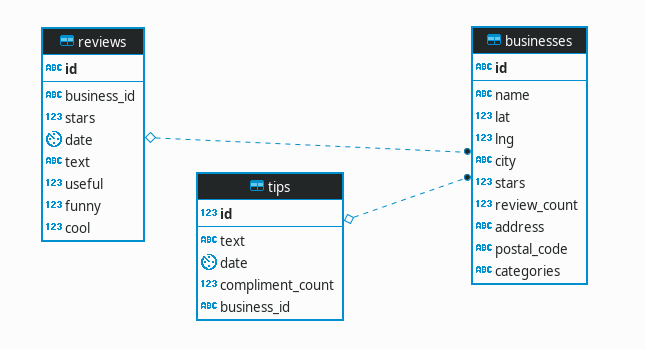
\includegraphics[width=130mm]{media/schema.png}
\end{center}
}

\subsection{\textgreek{Στατιστικά δεδομένων}}
    \textgreek{
    Μετά την εισαγωγή των δεδομένων στην βάση μας,
    με κατάλληλα ερωτήματα $SQL$ μπορούμε να βγάλουμε χρήσιμα στατιστικά
    προκειμένου να γίνει καλύτερη κατανόηση των δεδομένων μας.
    }

    \paragraph{\textgreek{Στατιστικά πόλεων}}
    \textgreek{
        Παρακάτω φαίνονται μερικά χρήσιμα στατιστικά ανα πόλη.

    \begin{enumerate}
        \item \textgreek{Αριθμός επιχειρήσεων ανά πόλη.}
        \item \textgreek{Αριθμός κριτικών ανά πόλη.}
        \item \textgreek{Μέσος αριθμός κριτικών και υποδείξεων.}
        \item \textgreek{Αριθμός υποδείξεων ($tips$) ανά πόλη.}
    \end{enumerate}

    \begin{center}
        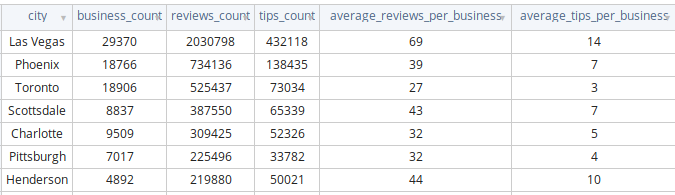
\includegraphics[width=130mm]{media/stats_table.png}
        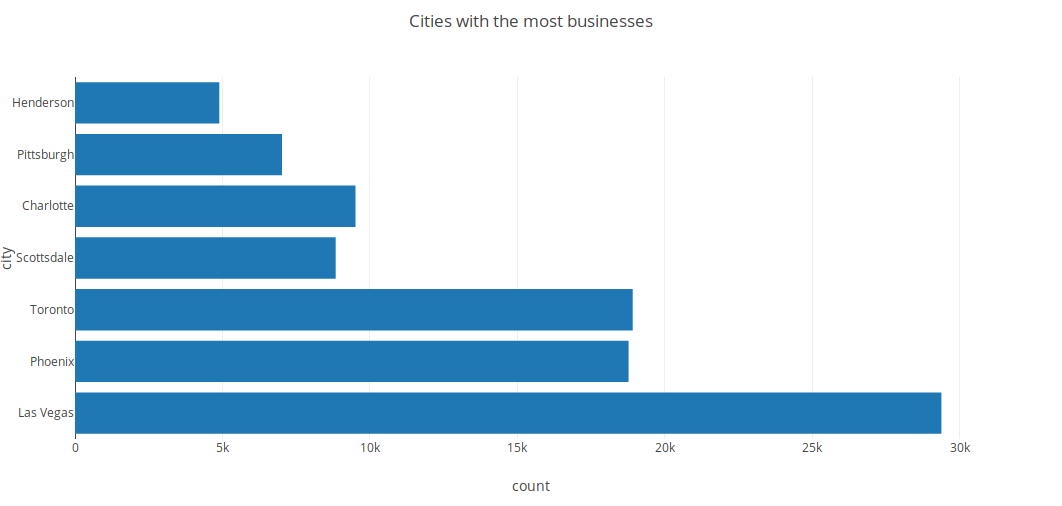
\includegraphics[width=130mm]{media/business_count_chart.png}
        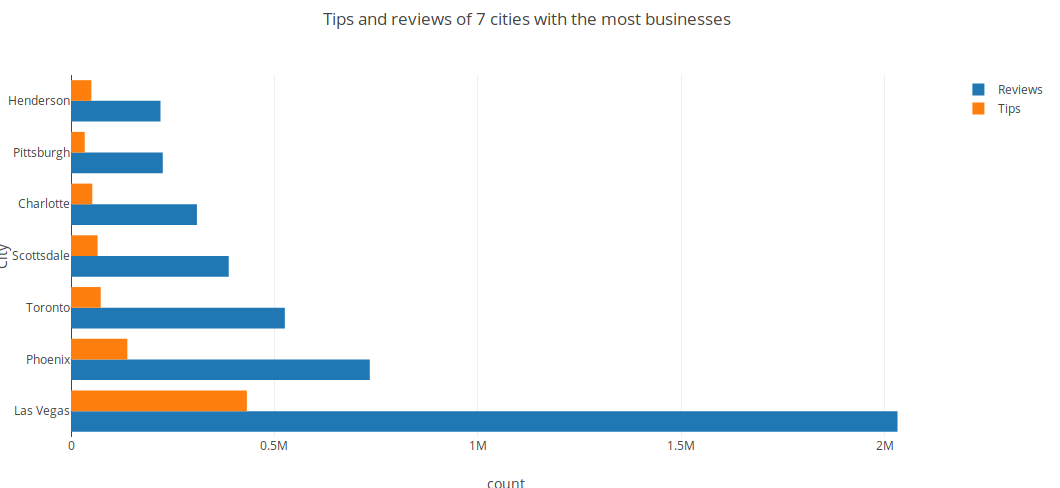
\includegraphics[width=130mm]{media/reviews_and_tips_chart.png}
    \end{center}

    \textgreek{
    Συνεπώς με βάση και με τα παραπάνω σχήματα επιλέξαμε την πόλη του $Las$ $Vegas$
    ως την πόλη πάνω στην οποία θα χτίσουμε την μηχανή αναζήτησής μας. Συγκεκριμένα
    έχει 29,400 επιχειρήσεις και συνολικα 2,470,000 κριτικές και υποδείξεις.
    }
}
